\documentclass[border=3pt]{standalone}
% Preâmbulo compartilhado pelos diagramas TikZ da aula 8 de Navegação (Implementação do RRT)
\usepackage[T1]{fontenc}
\usepackage[utf8]{inputenc}
\usepackage{lmodern}
\usepackage{amsmath}
\usepackage{xcolor}
\usepackage{tikz}
\usetikzlibrary{arrows.meta,angles,quotes,decorations.pathmorphing,decorations.pathreplacing,calc,
                positioning,shapes.geometric,shapes.misc,backgrounds,fit,
                math}

% Paleta (mesma dos SVGs originais)
\definecolor{dblue}{HTML}{2A5B8C}
\definecolor{dorange}{HTML}{B3541E}
\definecolor{dgreen}{HTML}{4A7C59}
\definecolor{dred}{HTML}{9C4B4B}
\definecolor{dcream}{HTML}{F4F1EA}
\definecolor{dshade}{HTML}{DDD7C9}

% Função gaussiana (não normalizada por padrão de escala visual)
\pgfmathdeclarefunction{gauss}{3}{%
  \pgfmathparse{1/(#3*sqrt(2*pi))*exp(-((#1-#2)^2)/(2*#3^2))}%
}

% Estilos comuns (prefixo d... para não colidir com chaves internas do pgf)
\tikzset{
  >={Stealth[length=2mm]},
  dguide/.style={gray!55, dashed, line width=0.4pt},
  daxis/.style={gray!60, line width=0.7pt, ->},
  dbody/.style={fill=black!3, draw=black!80, line width=1pt},
  dacc/.style={draw=dblue, line width=1pt},
  dlbl/.style={black!55, font=\small},
  dsub/.style={black!45, font=\footnotesize},
  dstate/.style={circle, draw=black!80, fill=dcream, line width=1pt,
                 minimum size=17mm, font=\large, inner sep=1pt},
  dobs/.style={circle, draw=black!80, fill=dshade, line width=1pt,
               minimum size=14mm, font=\large, inner sep=1pt},
  dbox/.style={rounded corners=2pt, draw=black!80, fill=dcream, line width=1pt,
               align=center, inner sep=6pt},
  dop/.style={circle, draw=black!80, fill=white, line width=1pt,
              minimum size=6mm, inner sep=0pt, font=\small},
  dtrans/.style={->, dblue, line width=1pt},
  dmeas/.style={->, dorange, line width=1pt},
  dcurve/.style={line width=1pt, dblue},
  dcurveb/.style={line width=1.4pt, dorange},
}

\begin{document}
\hyphenpenalty=10000 \exhyphenpenalty=10000 \tolerance=9999 \emergencystretch=3em
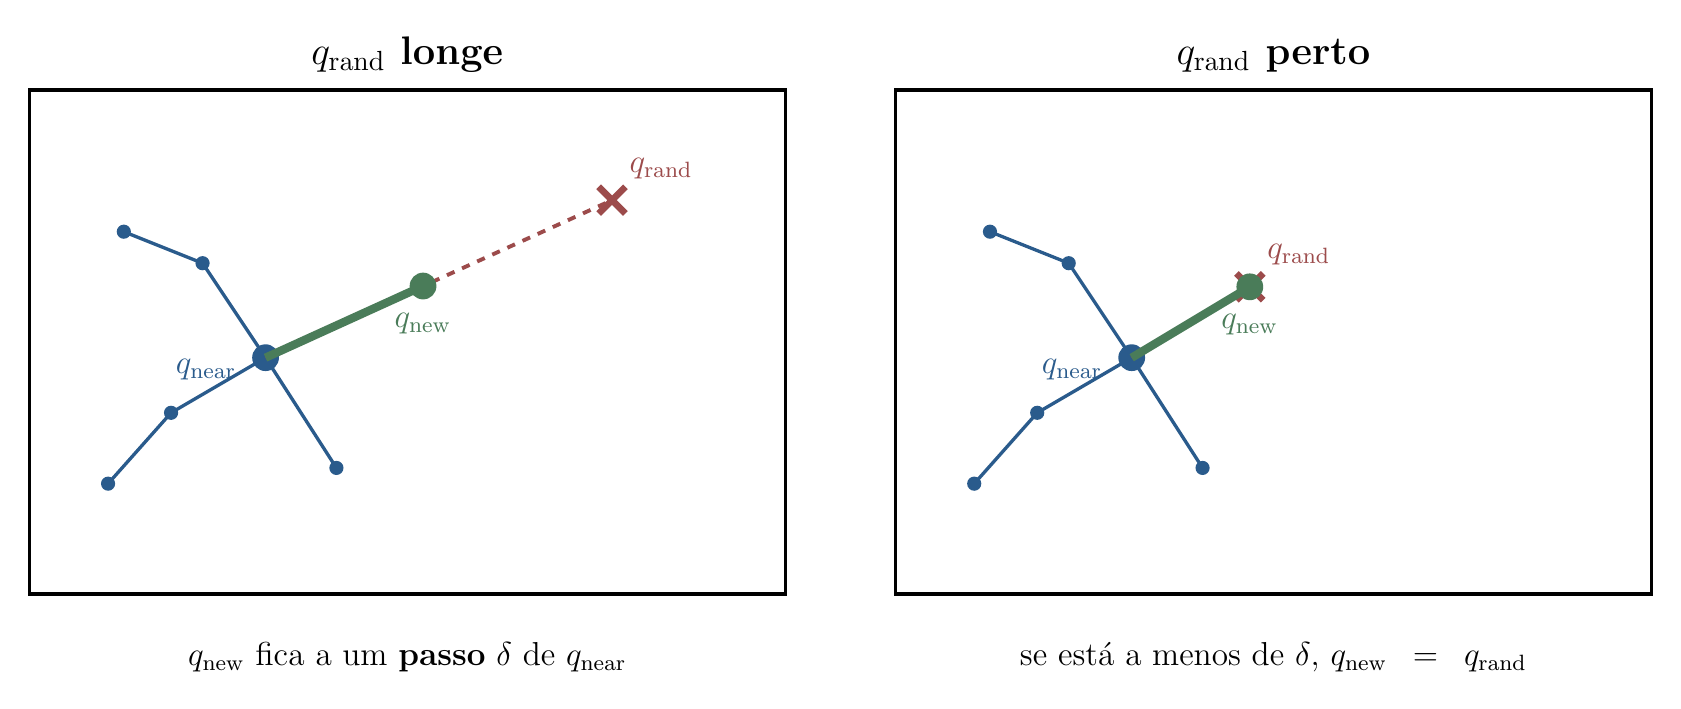
\begin{tikzpicture}[x=1cm,y=1cm]
\draw[line width=1.2pt, fill=white] (0.00,0) rectangle (9.60,6.4);
\draw[dblue, line width=1.2pt] (1.00,1.40) -- (1.80,2.30);
\draw[dblue, line width=1.2pt] (1.80,2.30) -- (3.00,3.00);
\draw[dblue, line width=1.2pt] (3.00,3.00) -- (2.20,4.20);
\draw[dblue, line width=1.2pt] (3.00,3.00) -- (3.90,1.60);
\draw[dblue, line width=1.2pt] (2.20,4.20) -- (1.20,4.60);
\fill[dblue] (1.00,1.40) circle (0.09);
\fill[dblue] (1.80,2.30) circle (0.09);
\fill[dblue] (3.00,3.00) circle (0.09);
\fill[dblue] (2.20,4.20) circle (0.09);
\fill[dblue] (3.90,1.60) circle (0.09);
\fill[dblue] (1.20,4.60) circle (0.09);
\fill[dblue] (3.00,3.00) circle (0.17); \node[font=\large\bfseries, text=dblue, anchor=east] at (2.75,2.85) {$q_{\mathrm{near}}$};
\draw[dred, line width=2.4pt] (7.23,4.83) -- (7.57,5.17) (7.23,5.17) -- (7.57,4.83);
\node[font=\large\bfseries, text=dred, anchor=south west] at (7.50,5.15) {$q_{\mathrm{rand}}$};
\draw[dred, dashed, line width=1.4pt] (3.00,3.00) -- (7.40,5.00);
\draw[dgreen, line width=3pt] (3.00,3.00) -- (5.00,3.91);
\fill[dgreen] (5.00,3.91) circle (0.17); \node[font=\large\bfseries, text=dgreen, anchor=north] at (5.00,3.69) {$q_{\mathrm{new}}$};
\node[font=\Large\bfseries, anchor=south] at (4.80,6.5) {$q_{\mathrm{rand}}$ longe};
\node[font=\large, text width=9.4cm, align=center] at (4.80,-0.8) {$q_{\mathrm{new}}$ fica a um \textbf{passo} $\delta$ de $q_{\mathrm{near}}$};
\draw[line width=1.2pt, fill=white] (11.00,0) rectangle (20.60,6.4);
\draw[dblue, line width=1.2pt] (12.00,1.40) -- (12.80,2.30);
\draw[dblue, line width=1.2pt] (12.80,2.30) -- (14.00,3.00);
\draw[dblue, line width=1.2pt] (14.00,3.00) -- (13.20,4.20);
\draw[dblue, line width=1.2pt] (14.00,3.00) -- (14.90,1.60);
\draw[dblue, line width=1.2pt] (13.20,4.20) -- (12.20,4.60);
\fill[dblue] (12.00,1.40) circle (0.09);
\fill[dblue] (12.80,2.30) circle (0.09);
\fill[dblue] (14.00,3.00) circle (0.09);
\fill[dblue] (13.20,4.20) circle (0.09);
\fill[dblue] (14.90,1.60) circle (0.09);
\fill[dblue] (12.20,4.60) circle (0.09);
\fill[dblue] (14.00,3.00) circle (0.17); \node[font=\large\bfseries, text=dblue, anchor=east] at (13.75,2.85) {$q_{\mathrm{near}}$};
\draw[dred, line width=2.4pt] (15.33,3.73) -- (15.67,4.07) (15.33,4.07) -- (15.67,3.73);
\node[font=\large\bfseries, text=dred, anchor=south west] at (15.60,4.05) {$q_{\mathrm{rand}}$};
\draw[dred, dashed, line width=1.4pt] (14.00,3.00) -- (15.50,3.90);
\draw[dgreen, line width=3pt] (14.00,3.00) -- (15.50,3.90);
\fill[dgreen] (15.50,3.90) circle (0.17); \node[font=\large\bfseries, text=dgreen, anchor=north] at (15.50,3.68) {$q_{\mathrm{new}}$};
\node[font=\Large\bfseries, anchor=south] at (15.80,6.5) {$q_{\mathrm{rand}}$ perto};
\node[font=\large, text width=9.4cm, align=center] at (15.80,-0.8) {se está a menos de $\delta$, $q_{\mathrm{new}}=q_{\mathrm{rand}}$};
\end{tikzpicture}
\end{document}
